% mainfile: ../../main.tex
\chapter{Characterization and improvements of the optical path}\label{ch:setup:optics}
\AutoLettrine{The} confocal microscope integrated into a millikelvin-temperature cryogen-free \gls{dr} accommodating free-space optical measurements together with DC and AC electrical control was designed and set up by \citeauthor{Descamps2024}~\cite{Descamps2021,Descamps2024}.
In this chapter, I lay out improvements to the design to improve the optical efficiency of the microscope.
I review the relevant relationships between optical parameters, estimate the maximum expected efficiency, and compare it to measurements.
Furthermore, I characterize the cross-polarization extinction and outline various schemes I established to automatically control the motorized stages regulating the excitation power and rejection as well as the diffraction grating spectrometer and \gls{ccd}.
Lastly, I demonstrate the setup's efficacy to measure photon anti-bunching in a \g2 measurement on self-assembled quantum dots in \ch{InGaAs}.

\section{Light coupling}\label{sec:setup:optics:coupling}
While the microscope arrangement on top of and inside the cryostat is free space optics to enable imaging of the sample, illumination and collected light are routed to and from the optical table using \glspl{smf}.
Convenience aside, for the illumination this is a natural choice since the guiding mode of these fibers very closely approximates the fundamental \tem{00} laser mode~\cite{Kowalevicz2006}.
For the collected light, it is less obvious that a \gls{smf} is the best choice.
Coupling light -- of any mode profile -- in and out of fibers invariably incurs losses.
Because of the small mode field diameters on the order of a few micrometers, aligning the optics for coupling is a sensitive task and subject to external disturbances.
Moreover, even for perfect mode matching and alignment, there are reflection losses on the percent level.
On \cpageref{par:setup:optics:coupling:detection}, I discuss the coupling of collected light into the \gls{smf} in more detail.
Despite these loss mechanisms, the single-mode character of the detection fiber is crucial to the microscope's operation because the cross-polarization extinction critically relies on the spatial filtering of the reflected mode by the fiber~\cite{Benelajla2021,Steindl2023}.
I discuss the cross-polarization extinction in more detail in \cref{subsec:sec:optics:coupling:rejection}.

\subsection{Choosing lenses}\label{subsec:setup:optics:coupling:lenses}

\begin{marginfigure}
    \begin{tikzpicture}[
    scale=2,%
    font=\footnotesize,%
    thick,%
    symmetryaxis/.style = {RWTHblack50,thin,dash dot},%
    lens/.style = {thick,<->},%
    optics/.style = {thick,black},%
    window/.style = {RWTHblue75,fill=RWTHblue25,text=black,opacity=0.75},%
    cryostat/.style = {RWTHblack75,thin,text=black},%
    midarrow1/.style = {postaction=decorate, decoration={markings,mark=at position 0.15 with \arrow{stealth}}},%
    midarrow2/.style = {postaction=decorate, decoration={markings,mark=at position 0.85 with \arrow{stealth}}},%
    midarrow/.style = {midarrow1, midarrow2},%
]    % requires libraries angle,quotes,calc,decorations.markings

    \ifdefined\CA
    \else
        \newlength\CA
    \fi
    \ifdefined\f
    \else
        \newlength\f
    \fi
    \ifdefined\dx
    \else
        \newlength\dx
    \fi
    \setlength\CA{0.25cm}
    \setlength\f{0.4cm}
    \setlength\dx{0.25cm}

    \coordinate (origin) at (0, 0);
    \coordinate (bs1) at (0, 0);
    \coordinate (bs2) at (0, -1);
    \coordinate (window) at ($(bs2) + (0, -0.8)$);
    \coordinate (objective) at ($(window) + (0, -1.5)$);

    \coordinate (detection-halfwave) at ($(bs1) + (0, 0.6)$);
    \coordinate (analyzer) at ($(detection-halfwave) + (0, 1*\dx)$);
    \coordinate (detection-ocular) at ($(detection-halfwave) + (0, 2*\dx)$);

    \coordinate (quarterwave) at ($(bs1) + (0.6, 0)$);
    \coordinate (excitation-halfwave) at ($(quarterwave) + (1*\dx, 0)$);
    \coordinate (polarizer) at ($(quarterwave) + (2*\dx, 0)$);
    \coordinate (excitation-ocular) at ($(quarterwave) + (3*\dx, 0)$);

    \coordinate (cmos-ocular) at ($(bs2) + (0.6, 0) + (3*\dx, 0)$);

    \coordinate (source) at ($(objective) - (0, \f)$);
    \coordinate (detection-fiber) at ($(detection-ocular) + (0, \f)$);
    \coordinate (excitation-fiber) at ($(excitation-ocular) + (\f, 0)$);
    \coordinate (cmos) at ($(cmos-ocular) + (\f, 0)$);

    % Symmetry axes
    \draw[symmetryaxis]
        ($(bs1) - (\CA*2,0)$)
        -- ($(excitation-fiber) + (\f/4,0)$)
    ;
    \draw[symmetryaxis]
        ($(bs2) - (\CA*2,0)$)
        -- ($(cmos) + (\f/4,0)$)
    ;
    \draw[symmetryaxis]
        ($(source) - (0, \f/4)$)
        -- ($(detection-fiber) + (0, \f/4)$)
    ;

    % Cryostat
    \draw[cryostat]
        ($(window) - (1.5*\CA, -0.025)$)
        -- ++($(-\f/2, 0)$)
        -- ($(source) - (1.5*\CA + \f/2, \f/2)$)
        -- ++($(3*\CA + \f, 0)$)
        -- ($(window) + (1.5*\CA + \f/2, 0.025)$) node[below,midway,rotate=90,xshift=5mm] {Cryostat}
        -- ++($(-\f/2, 0)$)
    ;

    % Beamsplitters
    \draw
        ($(bs1) - (1.5*\CA, 1.5*\CA)$) node[below left,xshift=2.1mm] {\acrshort{bs}1}
        -- ++($(3*\CA, 3*\CA)$)
    ;
    \draw[dashed]
        ($(bs2) - (1.5*\CA, 1.5*\CA)$) node[below left,xshift=2.1mm] {\acrshort{bs}2}
        -- ++($(3*\CA, 3*\CA)$)
    ;

    % Lenses
    \draw[lens]
        ($(objective) - (1.5\CA, 0)$)
        -- ++($(3*\CA, 0)$) node[right] {O}
    ;
    \draw[lens]
        ($(detection-ocular) - (1.5\CA, 0)$)
        -- ++($(3*\CA, 0)$) node[right] {D}
    ;
    \draw[lens]
        ($(excitation-ocular) + (0, 1.5\CA)$)
        -- ++($(0, -3*\CA)$) node[below] {E}
    ;
    \draw[lens]
        ($(cmos-ocular) + (0, 1.5\CA)$)
        -- ++($(0, -3*\CA)$) node[below] {C}
    ;

    % Optical elements
    \draw[optics,dashed]
        ($(detection-halfwave) - (1.5*\CA, 0)$)
        -- ++($(3*\CA, 0)$) node[right] {\halfwave}
    ;
    \draw[optics]
        ($(excitation-halfwave) + (0, 1.5*\CA)$)
        -- ++($(0, -3*\CA)$) node[below] {\halfwave}
    ;
    \draw[optics]
        ($(quarterwave) + (0, 1.5*\CA)$)
        -- ++($(0, -3*\CA)$) node[below] {\quarterwave}
    ;
    \draw[optics]
        ($(polarizer) + (0, 1.5*\CA)$)
        -- ++($(0, -3*\CA)$) node[below] {P}
    ;
    \draw[optics]
        ($(analyzer) - (1.5*\CA, 0)$)
        -- ++($(3*\CA, 0)$) node[right] {A}
    ;

    % Excitation beam
    \draw[midarrow,RWTHred100]
        (excitation-fiber)
        -- ++($(-\f, -\CA)$)
        -- ($(bs1) - (\CA, \CA)$)
        -- ($(-\CA, 0) + (objective)$)
        -- (source)
    ;
    % CMOS beam
    \draw[midarrow2,RWTHbordeaux100,dashed]
        (source)
        -- ++($(\CA, \f)$)
        -- ($(bs2) + (\CA, \CA)$)
        -- ($(cmos-ocular) + (0, \CA)$)
        -- (cmos)
    ;
    % Detection beam
    \draw[midarrow,RWTHbordeaux100]
        (source)
        -- ++($(\CA, \f)$)
        -- ($(\CA, 0) + (detection-ocular)$)
        -- ++($(-\CA, \f)$)
    ;

    % Windows
    \draw[window]
        ($(window) - (1.5*\CA, 0)$)
        rectangle ($(window) + (1.5*\CA, 0.05)$) %node[right] {Window}
    ;

\end{tikzpicture}

    \caption[\imgsource{img/tikz/setup/optical_path.tex}]{
        Reduced sketch of the microscope optical path.
        A Gaussian beam is launched from a \gls{smf} and collimated by the excitation ocular (E).
        It is polarized (P), passes \halfwave- and \quarterwave-plates, and is reflected into the cryostat by a 90:10 \acrfull{bs}.
        An objective lens (O) focuses the beam onto the sample and collects and collimates the emitted light.
        It exits the cryostat, is transmitted through the \gls{bs} and an analyzer (A) before being focused into the \gls{smf} by the detection ocular (D).
    }
    \label{fig:setup:optics:optical_path}
\end{marginfigure}

\Cref{fig:setup:optics:optical_path} shows a sketch of the free space optical path.
There are three lenses that need to fulfil different tasks.
First, the excitation ocular (E), which collimates the Gaussian beam launched from the fiber.
Next, the objective lens (O), which focuses the beam onto the sample and at the same time collects and collimates the reflected and emitted light.
Finally, the collected light is focused by the detection ocular (D) into another fiber for spectral analysis.
Since Gaussian beams behave fundamentally differently to geometrical optics, there are different requirements for the lens specifications.
In the following, I will review the different beam behaviors and outline the rationale behind the choices made for the lenses.

The fundamental Gaussian \tem{00} mode has the rotationally symmetric electric field profile~\cite{Yariv1989}
\begin{equation}\label{eq:setup:optics:coupling:efield:tem00}
E(\rho, z) = E_0\frac{w_0}{w(z)}\exp\left\lbrace -\i\left[kz - \arctan(\frac{z}{z_0})\right] - \rho^2\left[\frac{1}{w(z)^2} + \frac{ik}{2 R(z)}\right]\right\rbrace
\end{equation}
with the beam waist radius $w_0$, the beam's $1/\e$-radius
\begin{equation}\label{eq:setup:optics:coupling:gaussian:radius}
    w(z)^2 = w_0^2\left(1 + \frac{z^2}{z_0^2}\right),
\end{equation}
the wavefront radius of curvature
\begin{equation}
    R(z) = z\left(1 + \frac{z_0^2}{z^2}\right),
\end{equation}
the Rayleigh range
\begin{equation}\label{eq:setup:optics:coupling:gaussian:rayleigh_range}
    z_0 = \frac{\pi w_0^2}{\lambda},
\end{equation}
and where $z=0$ at the beam waist as well as $\lambda = \lambda_0/n$ the wavelength in the propagating medium.
For a \gls{smf}, the \gls{mfd} is $2 w_0$ and a beam launched from it expands according to \cref{eq:setup:optics:coupling:gaussian:radius} with $z=0$ in its end face.

The Rayleigh range determines the the extent of the mode's near field.
At $z=z_0$, the diameter of the beam is $w(z_0) = w_0\sqrt{2}$.
In the far field, the beam divergence is given by
\begin{equation}\label{eq:setup:optics:coupling:gaussian:divergence}
    \theta_{\mr{beam}} = \arctan(\frac{w_0}{z_0}) \approx \frac{\lambda}{\pi w_0}.
\end{equation}
Collimating a Gaussian beam emerging from a \gls{smf} thus requires matching $\theta_{\mr{beam}}$ with the \gls{na} of the lens such that $\mr{\acrshort{na}}\geq\sin\theta_{\mr{beam}}$.
Conversely, coupling a beam into a \gls{smf} requires matching the fiber's \gls{mfd} to the spot size, which is constrained by diffraction.
From \cref{eq:setup:optics:coupling:gaussian:divergence} we find, by setting $w = f\tan\theta_{\mr{beam}}$, the rule-of-thumb
\begin{equation}\label{eq:setup:optics:coupling:gaussian:diffraction_limit}
    w_0 \approx \frac{\lambda f}{\pi w}
\end{equation}
where $w$ is the beam radius at the focusing lens.\sidenote{
    Note that this disregards diffraction at the aperture and is thus only a good approximation for a \acrshort{ca} well larger than $w$.
}
For non-Gaussian beams one typically quotes the radius of the first Airy disk assuming a flattop profile~\cite{Hecht2017},
\begin{equation}\label{eq:setup:optics:coupling:flattop:diffraction_limit}
    w_0 \approx 1.22\frac{\lambda f}{2 w},
\end{equation}
where $w$ is the radius of the lens aperture.

\paragraph{Excitation path}
Now, for as small a spot on the sample as possible, we conclude from \cref{eq:setup:optics:coupling:gaussian:diffraction_limit} that we should choose an objective lens with a small focal length \fob (large \acrshort{na}) and illuminate it with a beam with a large diameter $2 w$.
As the lens diameter and hence the \acrfull{ca}\sidenote{
    The \gls{ca} is the diameter over which the lens specifications hold.
    Outside this diameter, light may still be transmitted but is not guaranteed to behave according to the lens design.
}
is constrained by the available space in the sample puck, the best lens was found to be \objectivelens~\cite{Thorlabs354330} with $\fob = \qty{3.1}{\milli\meter}$, $\mr{\acrshort{na}} = \num{0.7}$, and infinity-side $\mr{\acrshort{ca}} = \qty{5}{\milli\meter}$.\sidenote{
    A lens with even higher \gls{na} exists~\cite{Lightpath355330} but I found it to have too short a \gls{wd} to put our flip-chipped samples into focus.
    Samples with a different mounting strategy might benefit from the slightly increased focusing power of that lens.
}
Having chosen the objective lens, we can next select the excitation ocular to match the beam diameter.
For our typical excitation wavelengths around \qty{800}{\nano\meter}, the best-matching \gls{smf} has $\mr{\acrshort{mfd}} = 2 w_0 = \qty{5}{\micro\meter}$~\cite{Thorlabs780HP}.
Again using \cref{eq:setup:optics:coupling:gaussian:diffraction_limit} and solving for $f$, we find $\foc = \flatfrac{\pi w_0 w}{\lambda} \approx \qty{24.5}{\milli\meter}$ when setting $w = \flatfrac{\mr{\acrshort{ca}}}{2}$.
Since $w$ specifies the $\flatfrac{1}{e}$-radius of the beam, we should choose a lens resulting in a collimated beam diameter that is smaller than the \gls{ca}, \ie, a shorter focal length.
The lens that best matches this requirement is \ocularlens~\cite{ThorlabsA280TM} with $\foc = \qty{18.4}{\milli\meter}$, resulting in a collimated beam diameter of $2 w \approx\qty{3.8}{\milli\meter}$.
Collimating the Gaussian beam launched from a \gls{smf} may be viewed as transforming the beam waist $w_0\to w$, implying that the Rayleigh range after collimation is $z_0\approx\qty{13}{\meter}$ (\cref{eq:setup:optics:coupling:gaussian:rayleigh_range}), and the objective lens at a distance of $z\sim\qty{1.5}{\meter}$ is well in the beam's near field with negligible divergence (\cf \cref{eq:setup:optics:coupling:gaussian:radius}).
With the beam diameter and focal lengths set, we can compute the expected spot size to be $2 w_0\approx\qty{0.84}{\micro\meter}$.
In \cref{subsec:setup:optics:coupling:imaging} and \cref{sec:setup:vibrations:optic}, I compare this value to measurements.

\begin{figure*}
    \centering
    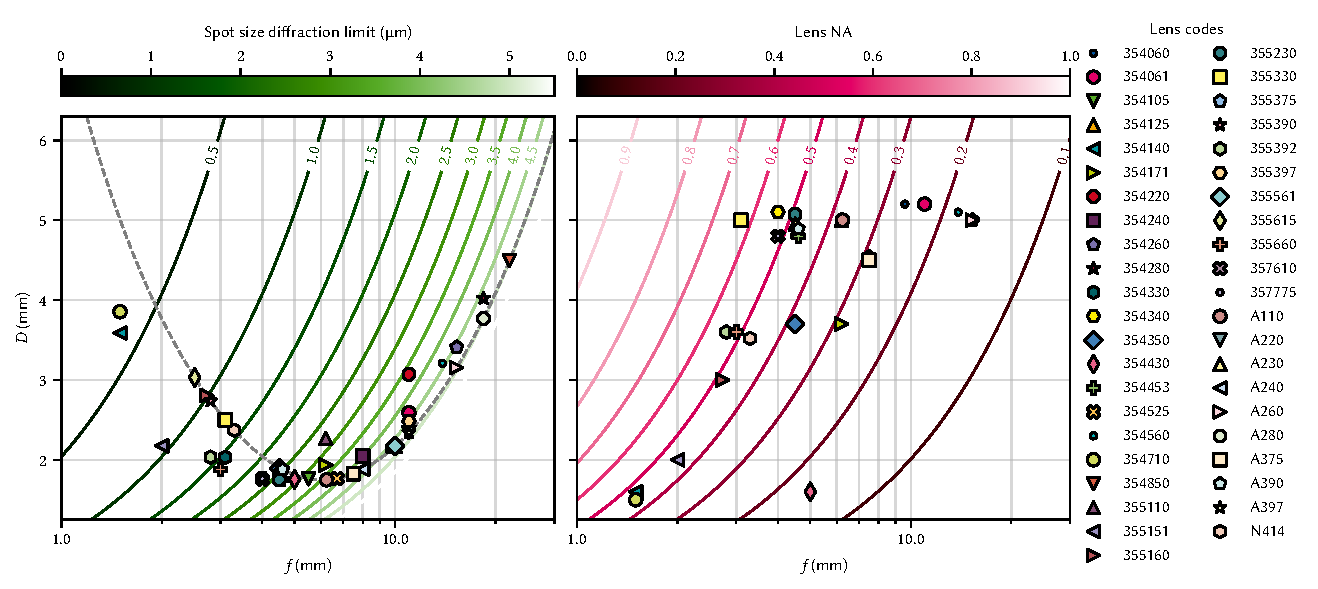
\includegraphics{img/pdf/setup/choosing}
    \caption[\imgsource{img/py/setup/single_mode_fiber_coupling.py}]{
        % TODO
    }
    \label{fig:setup:optics:coupling:lenses}
\end{figure*}

We have thus far addressed illumination of the sample with Gaussian laser light.
What now remains to deal with is the reverse direction; that is, collection of the emitted photoluminescence and focusing it into a \gls{smf} using the detection ocular lens (\enquote{D} in \cref{fig:setup:optics:optical_path}).
Before turning our attention to that task, let us briefly compare the expected performance with the lenses chosen here to those chosen in \citer{Descamps2021}.
There, the ocular lens had a focal length of $\foc = \qty{6.2}{\milli\meter}$ and the objective lens $\fob = \qty{4.51}{\milli\meter}$.
With these parameters, we obtain a beam diameter of $2w \approx\qty{1.3}{\milli\meter}$ just after collimation and a Rayleigh range of $z_0\approx\qty{1.5}{\meter}$, implying that the beam broadens by $\sim\sqrt{2}$ by the time it arrives at the objective lens $z\sim\qty{1.5}{\meter}$ away.
This would result in a spot size of $2 w_0\approx\qty{1.3}{\micro\meter}$, roughly a factor of two larger than with the lenses we chose here.

\paragraph{Detection path}\label{par:setup:optics:coupling:detection}
In a confocal microscope geometry, light is collected using the same lens that is also used for illumination of the sample.
For excitation with a Gaussian laser beam but non-Gaussian radiation being emitted, this means that two different beam behaviors need to be matched, a task that is likely not possible to achieve completely.
In the case of photoluminescence in a pristine semiconductor \gls{qw}, the optical interband transitions are well described by in-plane dipole matrix elements~\cite{Gu2013}.
If, on the other, the light emerges from a \gls{pcc}, the far field pattern is close to a Gaussian mode and the considerations below need to be adjusted accordingly~\cite{Wu2024}.
Here, I discuss dipole emission from the \gls{qw}, which needs to be coupled into a \gls{smf} with near-Gaussian mode profile, invariably resulting in losses.
A detailed analysis of the electric field profile to compute the expected coupling efficiency from the sample into the \gls{smf} is beyond our scope here as it would require taking into account the full sample and lens geometries as well as diffraction, a task only possible by employing a full-fledged numerical optics simulation suite.
However, we can make some crude simplifications of the problem to estimate the order of magnitude of these effects.
To this end, I model the light source as a point dipole beneath the surface of a homogeneous slab of dielectric material and the real lenses as ideal thin lenses.
% TODO: maybe a book reference here instead

\begin{marginfigure}
    \begin{tikzpicture}[
    scale=2,%
    font=\footnotesize,%
    thick,%
    axis/.style={RWTHblack75,text=black},%
]
    % requires libraries angle,quotes,calc

    \newlength\CA
    \setlength\CA{1cm}
    \newlength\tick
    \setlength\tick{0.1cm}

    \coordinate (origin) at (0,0);
    \coordinate (dipole) at (0,-0.5);
    \coordinate (interfacemargin) at (0.25,0);
    \coordinate (lens) at (0,1);
    \coordinate (lensmargin) at ($(\CA,1)$);

    % Coordinate axes
    \draw[->,axis]
        (origin)
        -- ($(\CA,0) + (0.4,0)$) node[right] {$x$}
    ;
    \draw[->,axis]
        (0.0,-0.75)
        -- ($(lens) + (0,0.25)$) node[above] {$z$}
    ;
    % Xticks
    \draw[axis]
        (\CA,0)
        -- ++(0,-\tick) node[below] {$w$}
    ;
    % Yticks
    \draw[axis]
        (lens)
        -- ++(-\tick,0) node[left] {\fob}
        (origin)
        -- ++(-\tick,0) node[left] {$0$}
        (dipole)
        -- ++(-\tick,0) node[left] {$-d$}
    ;
    % Angles
    \draw[thin,axis]
        ($(interfacemargin) - (0,0.1)$)
        -- ++(0,0.5) node (beta) {}
    ;
    \pic[draw,"$\alpha$",angle eccentricity=1.5,axis]
        {angle = interfacemargin--dipole--origin}
    ;
    \pic[draw,"$\beta$",angle eccentricity=1.5,axis]
        {angle = lensmargin--interfacemargin--beta}
    ;

    % Lens and QW
    \draw[very thick]
        (lens)
        -- ++(1.25,0) node[right] {Ob.}
    ;
    \draw[dashed,RWTHblack75]
        ($(dipole) + (0,0.05)$)
        -- ++(1.25,0)
        ($(dipole) - (0,0.05)$)
        -- ++(1.25,0)
    ;
    \node[anchor=west] at ($(dipole) + (1.25,0)$) {\acrshort{qw}};

    % Margin beam
    \draw[->,RWTHred100]
        (dipole)
        -- (interfacemargin)
        -- (lensmargin)
        -- ++(0,0.25)
    ;
\end{tikzpicture}

    \caption[\imgsource{img/tikz/setup/emission.tex}]{
        Sketch of a light source located inside a dielectric medium ($z < 0, n > 1$) emitting light in the upwards direction to collection by an objective lens in air ($z > 0, n = 1$).
        The red line indicates the marginal ray of the lens with focal length \fob and \gls{ca} $2w$.
    }
    \label{fig:setup:optics:coupling:emission}
\end{marginfigure}

Consider the situation sketched in \cref{fig:setup:optics:coupling:emission}.
A dipole oriented along $x$ in the plane of a \ch{GaAs} \gls{qw} with refractive index $n$ buried at a depth $d$ beneath the surface of the sample emits light into the halfspace above it.
The emitted radiation has the electric field distribution~\cite{Griffiths2017}
\begin{equation}\label{eq:setup:optics:coupling:efield}
    E(x,y,z) = E_{0}\frac{\exp(\i k r)}{r}\cos\theta
\end{equation}
where $\theta=\arctan{\flatfrac{x}{z}}$, $r$ is the distance from the point dipole and $k=\flatfrac{2\pi}{\lambda}=\flatfrac{2\pi n}{\lambda_0}$ is the wavenumber in the medium.

The emitted light is refracted at the surface and we collect and collimate it with an objective lens (labelled \enquote{Ob.}) with $\mr{\acrshort{na}}=\sin\theta^\prime_\mr{m}$ at distance \fob above the surface of the sample, where \fob is the focal length and $\theta^\prime_\mr{m}$ the angle of the marginal ray.
The \gls{na} determines the maximum amount of light the objective lens can collect, and using Snell's law we can relate the angle of a ray outside the sample $\theta^\prime$ to the angle inside the sample $\theta$,
\begin{equation}\label{eq:setup:optics:coupling:snell}
    \sin\theta^\prime = n\sin\theta,
\end{equation}
with $n\approx 3.57$ at $\lambda_0=\qty{800}{\nano\meter}$ and $T=\qty{0}{\kelvin}$.
This yields $\theta_{\mr{m}} = \arcsin(\flatfrac{\mr{\acrshort{na}}}{n}) \approx\qty{11}{\degree}$ for the emission angle of the marginal ray inside the semiconductor, suggesting that \cref{eq:setup:optics:coupling:efield} is well approximated as a spherical wave since $\cos\theta_{\mr{m}}\approx 1-\theta_{\mr{m}}^2/2\approx 1$.
Indeed, the fraction of the emitted intensity $I(\theta)\propto\abs{E(\theta)}^2$ being collected by the objective lens, the \emph{collection efficiency}, is
\begin{equation}\label{eq:setup:optics:coupling:efficiency:collection}
    \begin{split}
        \eta_{\mr{c}} &= \frac{\iint_{\theta_{\mr{m}}}\dd{\Omega} I(\theta)}{\iint\dd{\Omega} I(\theta)}
                      = \frac{\int_{0}^{\theta_{\mr{m}}}\dd{\theta}\sin\theta\cos^2\theta}{\int_{0}^{\pi}\dd{\theta}\sin\theta\cos^2\theta} \\
                      &= \frac{1}{2}\left(1 - \left[1 - \left(\frac{\mr{\acrshort{na}}}{n}\right)^2\right]^{\flatfrac{3}{2}}\right)
    \end{split}
\end{equation}
which evaluates to only $\eta_{\mr{c}}\approx\qty{2.8}{\percent}$ for the objective lens's $\mr{\acrshort{na}}=\num{0.7}$.
Moreover, since $d\sim\qty{100}{\nano\meter}\ll\fob\sim\qty{1}{\milli\meter}$ and also $kd\ll 1$, the lateral extent of the light source as viewed from the objective lens is negligibly small and is well approximated by a point source right below the surface.

In order to determine the electric field amplitude as a function of position inside the lens with radius $w$, consider a light ray impinging on the surface at lateral position $x_0$.
Taking two points of the light ray at $(x_0-\Delta x, -\epsilon)$ some $\epsilon > 0$ below the surface and $(x_0 + \Delta x^\prime, +\epsilon)$ above, we can express the lateral shift due to refraction as
\begin{equation}
    \Delta x^{\prime} = \epsilon\tan\theta^{\prime} = \Delta x \frac{n\cos\theta}{\sqrt{1 - n^2\sin^2\theta}}
\end{equation}
with $\theta^{(\prime)} = \arctan(\Delta x^{(\prime)}/\epsilon)$ using standard trigonometric identities.
Thus, the coordinate $x$ of the electric field inside the semiconductor transforms to the coordinate $x^\prime$ outside the semiconductor as
\begin{equation}
    x\to x^{\prime} = x n \left[1 + \left(\frac{x}{z}\right)^2 - \left(\frac{nx}{z}\right)^2\right]^{-\frac{1}{2}},
\end{equation}
which we invert to obtain
\begin{equation}\label{eq:setup:optics:coupling:coordinate_trafo}
    x = \frac{z}{\sqrt{n^2\left[1 + (z/x^{\prime})^2\right] - 1}}.
\end{equation}

We now approximate the light source as a point source at $z=-\epsilon < 0$ emitting a spherical wave as discussed above and introduce cylindrical coordinates with $\rho^{\prime} = \sqrt{x^{\prime 2} + y^2}$ so that $r = \sqrt{\rho^{\prime 2} + z^2}$.
Plugging \cref{eq:setup:optics:coupling:coordinate_trafo} into \cref{eq:setup:optics:coupling:efield} then yields
\begin{equation}\label{eq:setup:optics:coupling:efield:lens}
    E(\rho^\prime,z) = E_0\frac{\exp(\i k z\zeta(\rho^{\prime}))}{z\zeta(\rho^{\prime})}
\end{equation}
with
\begin{equation}
    \zeta(\rho^{\prime}) = \sqrt{1 + \left(n^2\left[1 + (z/\rho^{\prime})^2\right] - 1\right)\inverse}
\end{equation}
for the electric field outside the semiconductor.
At the lens $\zeta\approx 1$ so that the field is actually more closely resembled by a plane rather than the original spherical wave.

\begin{marginfigure}
    \centering
    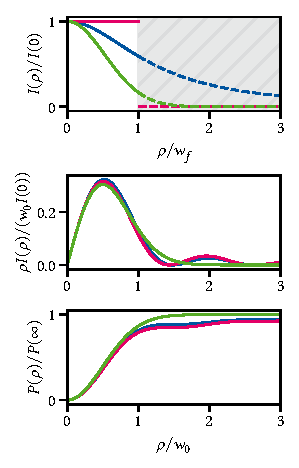
\includegraphics{img/pdf/setup/modes_1d}
    \caption[\imgsource{img/py/setup/single_mode_fiber_coupling.py}]{
        Electric field modes.
        Top: mode intensity of the light collected from the semiconductor at the objective lens plane (blue) in comparison to a flattop (green) and Gaussian \tem{00} mode with theoretical beam diameter after collimating with the ocular lens.
        $w$ is the lens \gls{ca} radius.
        Middle: diffraction pattern of the collimated beam approximated as a flattop when focusing onto the \gls{smf} end face with the ocular lens (green) and the fiber's guiding mode (magenta).
        The curves are scaled with the radial coordinate $\rho$ to highlight the Airy rings.
        Bottom: power encased by a circle with radius $\rho$, $P(\rho)\propto\int_0^{\rho}\dd{\rho^\prime} \rho^{\prime} I(\rho^{\prime})$.
    }
    \label{fig:setup:optics:coupling:modes_1d}
\end{marginfigure}

The radial intensity profile given by the absolute value square of \cref{eq:setup:optics:coupling:efield:lens} is shown in the upper panel of \cref{fig:setup:optics:coupling:modes_1d} together with a flattop (green) and a Gaussian (magenta) beam profile for comparison.
The intensity drops only by about \qty{2}{\percent} at the edge of the lens aperture, $\rho=w$.
We may thus expect non-negligible loss when coupling this beam into a \gls{smf} with a guiding mode very closely approximating the Gaussian \tem{00} mode whose electric field profile is given in \cref{eq:setup:optics:coupling:efield:tem00}~\cite{Kowalevicz2006}.

The light collected and collimated by the objective lens next passes through the ocular lens in the detection arm which focuses it into the \gls{smf}.
The image of the beam on the fiber end face is given by the Fraunhofer diffraction pattern generated by the (approximately) plane wave incident on the ocular lens aperture,\sidenote{
    We can safely neglect diffraction effects from the objective lens aperture.
    The Fraunhofer criterion $\flatfrac{b^2}{\lambda}$ with $b$ the aperture diameter is $\approx\qty{30}{\meter}$, implying the ocular lens at a distance of $\sim\qty{1}{\meter}$ is in the near field with many Fresnel zones where diffraction does not yet play a significant role~\cite{Hecht2017}.
}
resulting in the Airy disk~\cite{Hecht2017}
\begin{equation}\label{eq:setup:optics:coupling:airy}
    E(q) = E_0 2\pi w^2\frac{\exp(\i k \foc)}{\foc} \frac{J_1(\flatfrac{kwq}{\foc})}{\flatfrac{kwq}{\foc}},
\end{equation}
where $J_1(x)$ is Bessel function of order one and $q$ the radial coordinate in the image plane, \ie, the fiber end face.
\Cref{eq:setup:optics:coupling:airy} scaled with the radius $\rho$ is plotted in the middle panel of \cref{fig:setup:optics:coupling:modes_1d} together with the \gls{smf}'s guiding Gaussian mode.
While within the \gls{mfd} the two modes match quite well, a relevant amount of the power $P(\rho)\propto \int_0^{\rho}\dd{\rho^{\prime}} \rho^{\prime} I(\rho^{\prime})$ resides outside that radius as shown in the bottom panel of the same figure.

The mode matching efficiency is then given by the normalized spatial overlap of the light field ($E_{\mr{l}}$, \cref{eq:setup:optics:coupling:efield:lens}) and the fiber's guiding mode ($E_{\mr{f}}$, \cref{eq:setup:optics:coupling:efield:tem00})~\cite{Paschotta2005},
\begin{equation}\label{eq:setup:optics:coupling:efficiency:mode_matching}
    \eta_{\mr{m}} = \frac{\int\dd{S}\abs{E_{\mr{f}}(\rho)}^2\int\dd{S}\abs{E_{\mr{l}}(\rho)}^2}{\abs{\int\dd{S} E_{\mr{f}}(\rho) E_{\mr{l}}(\rho)}^2} \approx\qty{78}{\percent}
\end{equation}
for our parameters.
Together with the collection efficiency (\cref{eq:setup:optics:coupling:efficiency:collection}) and accounting for the transmittivity of the \gls{bs}, $T\approx\qty{87}{\percent}$,\sidenote{
    While the specifications of the beamsplitter are $T:R = \qty{90}{\percent}:\qty{10}{\percent}$, in reality $T:R\approx\qty{87}{\percent}:\qty{6}{\percent}$ which also varies slightly with polarization.
}
the \emph{optical efficiency}~\cite{Sze2007} from sample to fiber is thus
\begin{equation}
    \eta_{\mr{o}} = T\eta_{\mr{c}}\eta_{\mr{m}}\approx\qty{1.9}{\percent}.
\end{equation}

\subsection{Imaging the laser spot}\label{subsec:setup:optics:coupling:imaging}

\subsection{Cross-polarization extinction}\label{subsec:sec:optics:coupling:rejection}
